\section{Plugin Types}
\label{design:plugins}

We can already tell from the requirements that we must at least support two different plugin types, one for different cloud providers and one for different provisioning engines.
The former are required because we may want to provision into different cloud environments.
The latter are required because we might want to use different provisioning engines to do so.

The cloud provider plugins will be responsible for creating and removing resources in cloud environments and making them available for the user to configure and use.
This could be bare bone VMs (like AWS EC2 instances), or PaaS environments (like AWS Beanstalk).
We do not even have to constrain these plugins to cloud resources and can make them more generic, as long as we can run the plugin and get an IP address to a computing resource that we can use.
For example, we could also provide a plugin that starts and stops a VM on our local machine, which could be useful for quick and inexpensive local testing.
So a better name for these plugins would be \textit{resource plugins}.

The same line of thinking can be used on the provisioning engine plugins.
All that we care about is that we can get some software running on a given resource and that we get back an URL where we can find this software once it is up and running.
A better name for these plugins would therefore be \textit{application plugins}.

Now that we have resource plugins and application plugins, we should be able to provision the resource we need and use application plugins to install and run any software on it.
But there is a step in between provisioning the resource and installing the software that we are glancing over: We have to somehow communicate with the resource to be able to install something on it.
The communication functionality could be part of either the resource plugins or the application plugins, or it could be separated into independent communication plugins.
For the sake of efficiency and extensibility it would be best to use independent communication plugins.
For example, if a user wanted to add a new communication type that should be used to install x applications in y environments, they could do so by writing one new communication plugin, instead of adding the functionality x-times to all application plugins, or y-times to all resource plugins.
This would also reduce code duplication.
Therefore, a third plugin type is necessary: The \textit{communication plugins}.

The remote bootware also has to handle the initial provisioning of the workflow middleware, which involves calling a provisioning engine to tell it to start the provisioning process.
Because this has to be done differently for all provisioning engines, it would make sense to also package this functionality into plugins that can be interchanged.
We therefore introduce a fourth plugin type: The \textit{provision workflow middleware plugins}.
In \autoref{design:communication} we also introduced the notion of secondary communication channels realized by plugins.
We can generalize this into a more versatile fifth plugin type: The \textit{event plugins}.
These plugins are a bit less specific than the four other types.
They are not a part of the core bootware process but allow us to add functionality that reacts to (or creates) events inside the bootware for other purposes like, for example, logging.
How the actual event system used by these plugins will be implemented will be discussed in \autoref{design:internalcomm}.

With this fifth plugin type we have now covered all plugin types we will need.
Next, we present some examples of how the different plugin types will work together.
Then, we will describe each plugin type in more detail, starting with the common operations that all plugin types have to implement.

\subsection{Examples}

\autoref{image:plugin_process} shows an overview over the basic process involving the plugins.
The event plugins were omitted because they are not an essential part of this process.
In step one, the bootware calls a resource plugin to create a new resource instance, for example a VM.
Then, in step two, it creates a communication channel to this instance using a communication plugin.
This communication channel is then used in step three by an application plugin to install an application on the instance.
The fourth step is only executed when the remote bootware provisions the workflow middleware.
Here, a provision workflow middleware plugin can call this application, in this case a provisioning engine, to provision a workflow middleware.
How the bootware knows which plugins it should call is determined by the context which is explained in \autoref{design:context}.

\autoref{image:plugin_process_2} shows the same process but with an exemplary selection of specific plugin instances.
In this case, an Amazon plugin is used in step one to create an EC2 instance.
In step two, a SSH plugin creates a connection to this EC2 instance.
Over this SSH connection, an OpenTOSCA plugin installs OpenTOSCA on the EC2 instance, as shown in step three.
Finally, in step four, a call OpenTOSCA plugin calls the just deployed OpenTOSCA container to provision the workflow middleware.
For another combination of plugins, the process might look like \autoref{image:plugin_process_3}.
Here, a Chef server is installed on an Azure VM over a \nom{remote desktop connection}{RDC}.
The Chef server is then used to provision the workflow middleware.

\begin{figure}[!htbp]
	\centering
	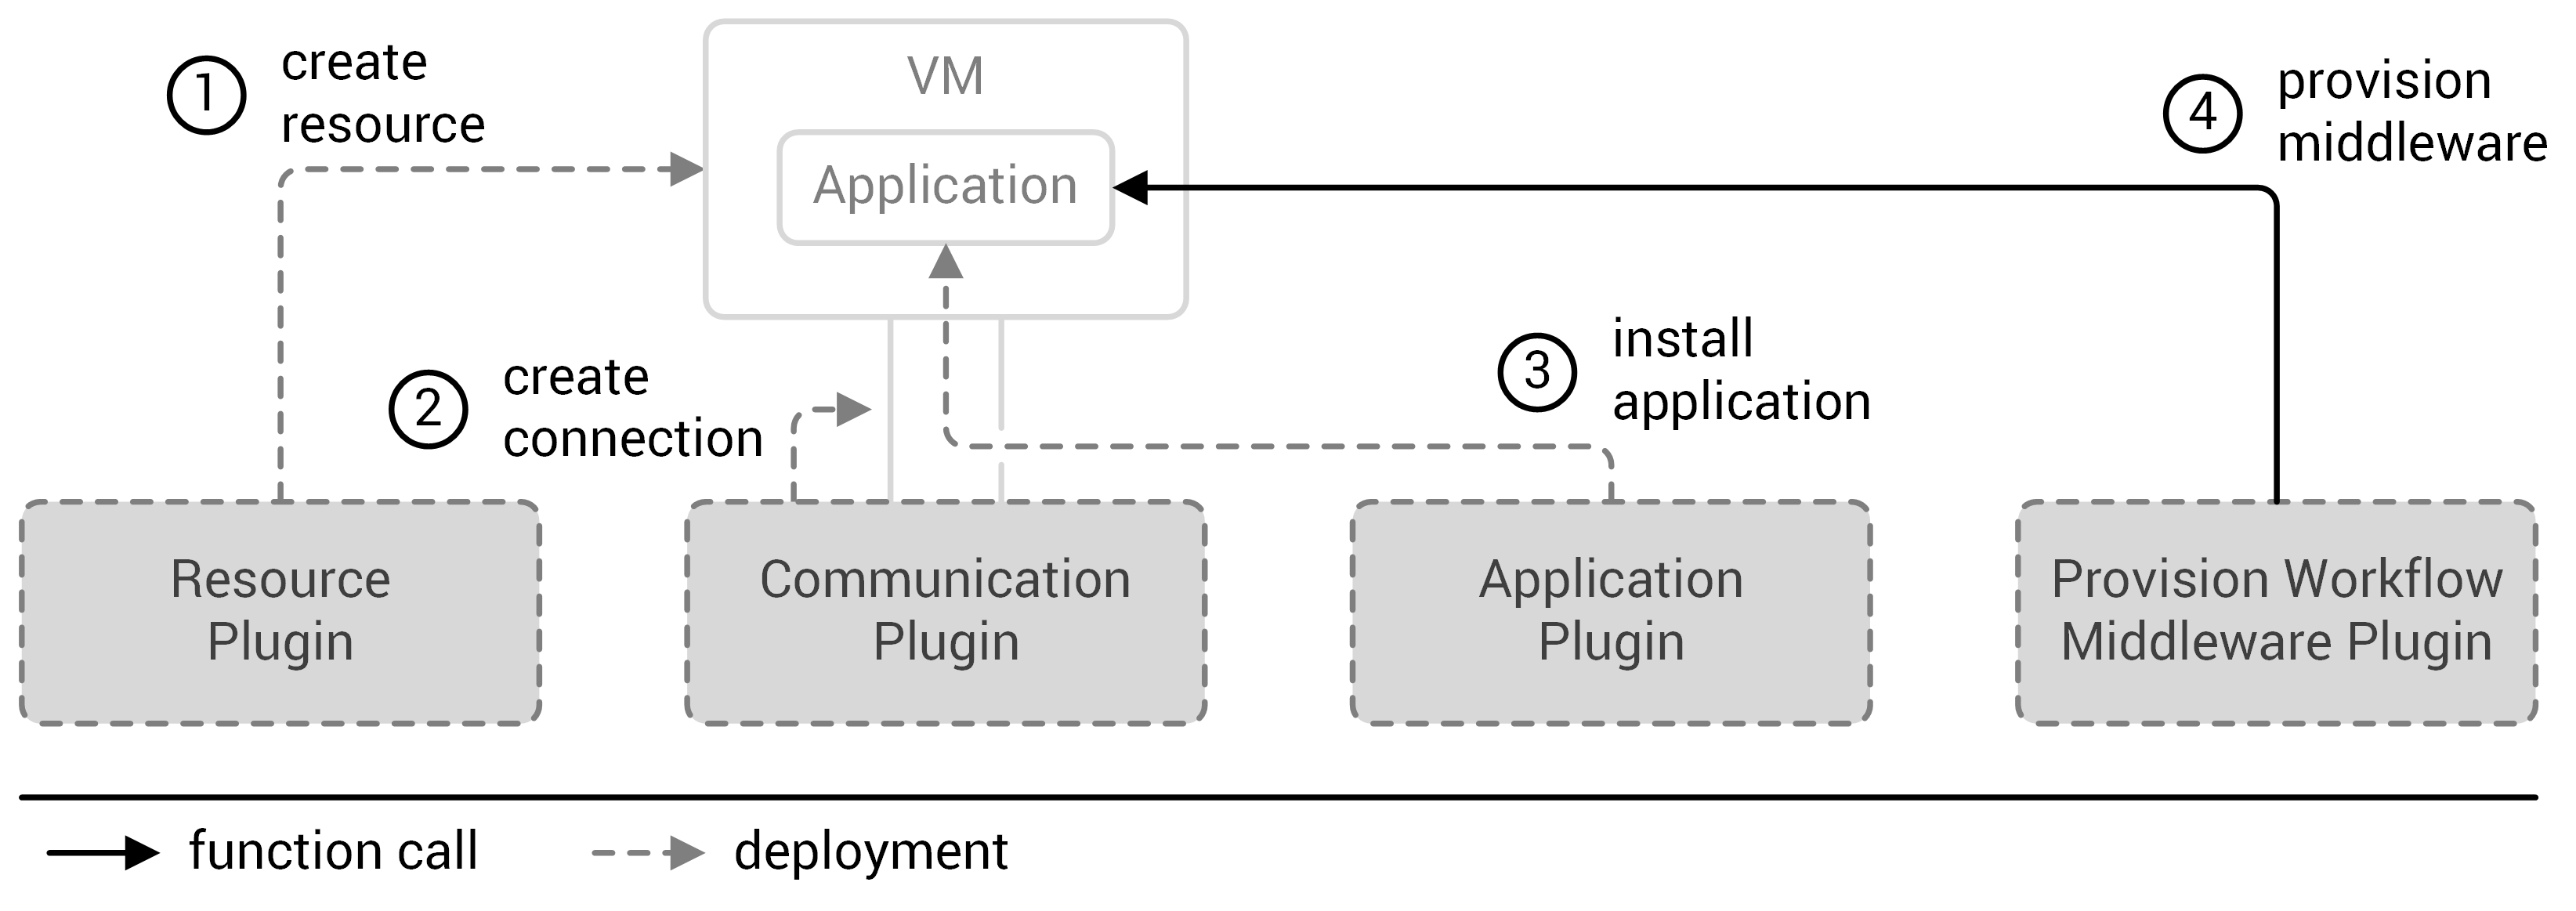
\includegraphics[resolution=600]{design/assets/plugin_process}
	\caption{Simplified overview of the plugin process.}
	\label{image:plugin_process}
\end{figure}

\vspace{1.0cm}

\begin{figure}[!htbp]
	\centering
	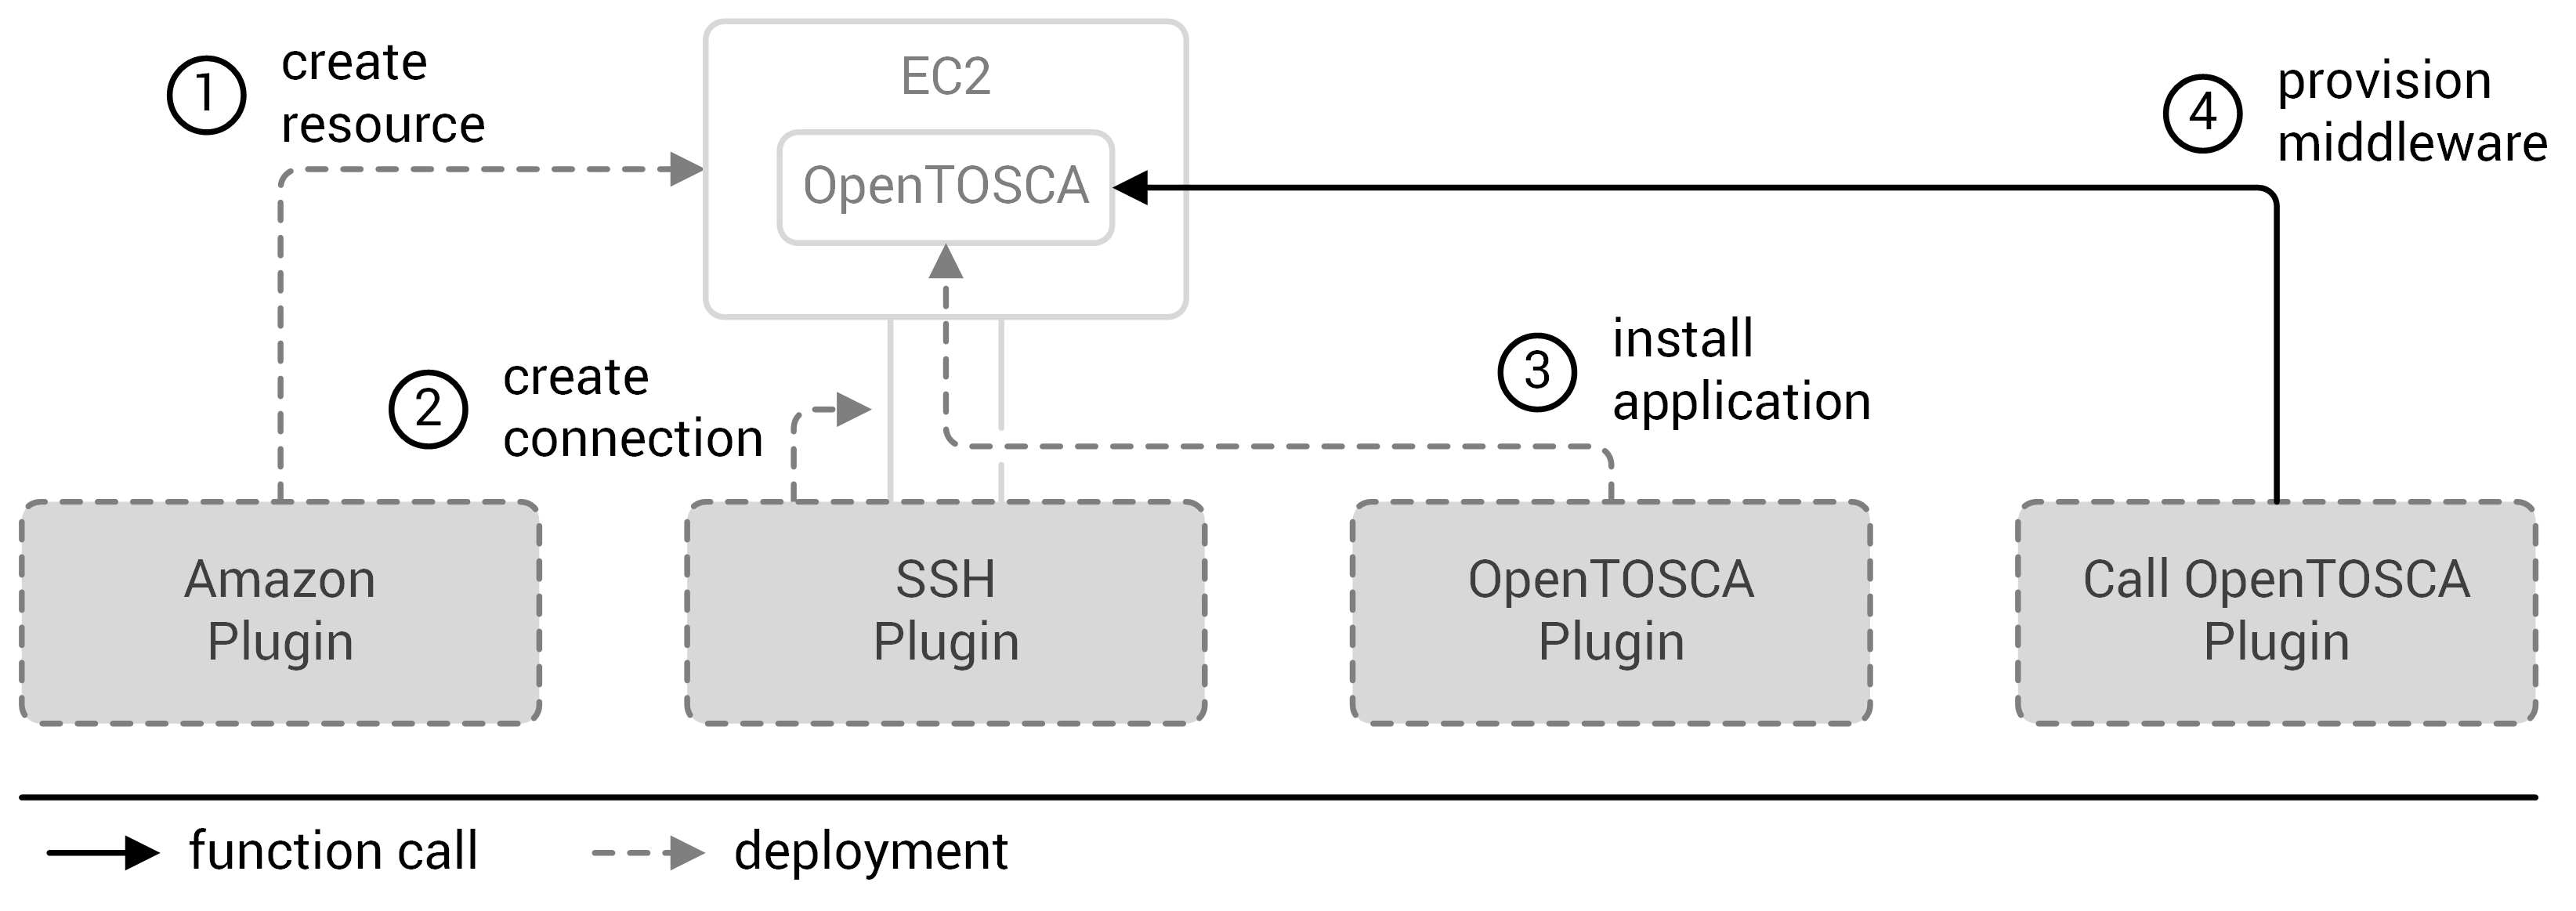
\includegraphics[resolution=600]{design/assets/plugin_process_2}
	\caption{Exemplary plugin process for Amazon and OpenTOSCA.}
	\label{image:plugin_process_2}
\end{figure}

\vspace{1.0cm}

\begin{figure}[!htbp]
	\centering
	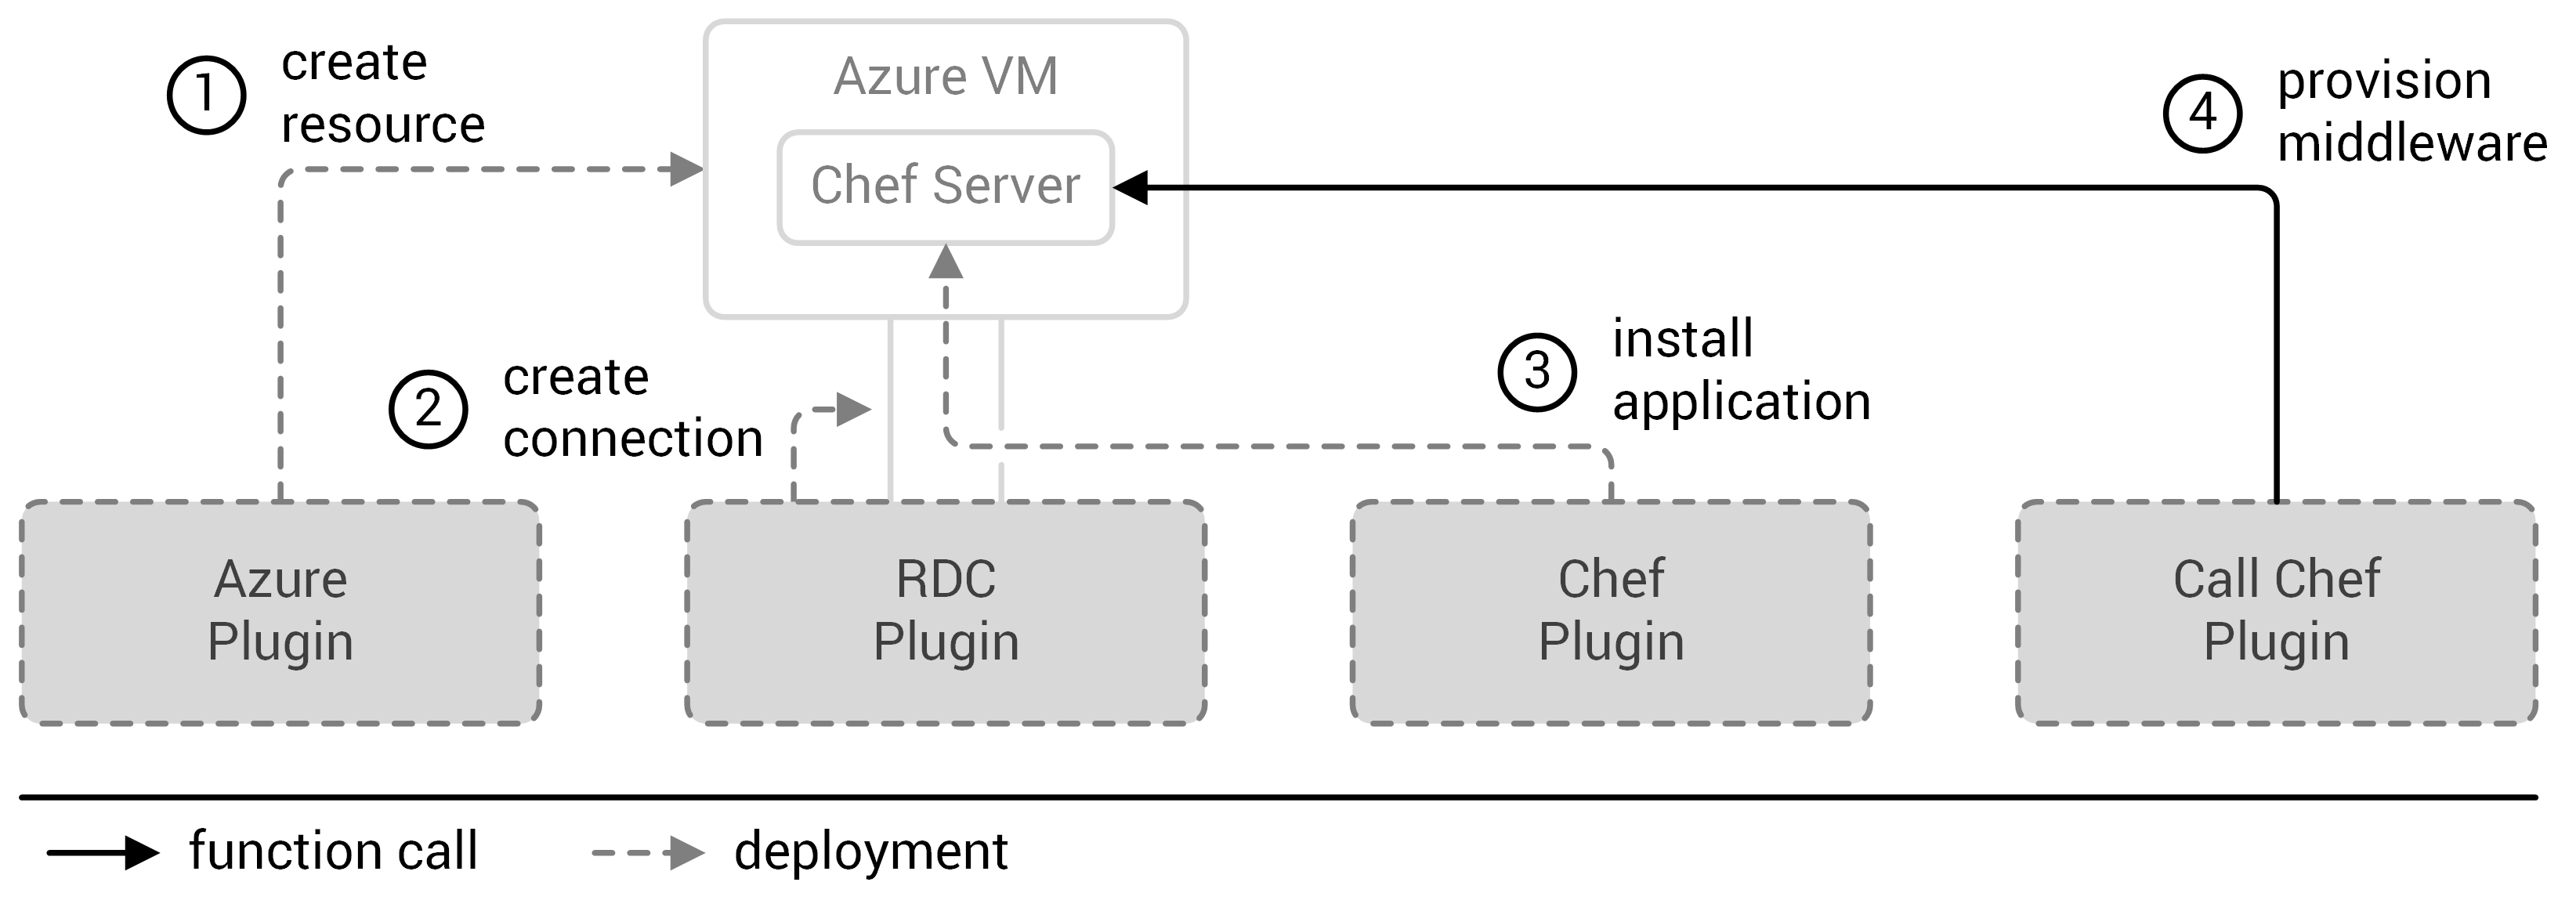
\includegraphics[resolution=600]{design/assets/plugin_process_3}
	\caption{Exemplary plugin process for Azure and Chef.}
	\label{image:plugin_process_3}
\end{figure}

\subsection{Common Operations}

\autoref{table:all_plugins} shows the two common operations that all plugin types must implement.
The initialize operation is called by the plugin manager when it loads a plugin.
This operation can be used by plugin authors to initialize the plugin, for example by creating internal objects that will be used by other plugin operations later on.
It takes a configuration object as parameter, which is taken from the request context.
This allows the plugins to be configured from the outside if necessary.
The shutdown operation is called by the plugin manager when it unloads a plugin.
It can be useful to clean up plugin resources before the plugin is removed, for example by deleting temporary files or closing a communication channel.

\vspace*{\baselineskip}
\begingroup
	\centering
	\captionsetup{type=table}
	\renewcommand{\arraystretch}{2}
	\begin{tabu}[!htbp]{X[2,r]X[2,c]X[2,c]X[6,l]}

			\multicolumn{1}{c}{\textbf{Operation}}
		& \multicolumn{1}{c}{\textbf{Input}}
		& \multicolumn{1}{c}{\textbf{Output}}
		& \multicolumn{1}{c}{\textbf{Description}} \\

		\tabucline[0.5pt]{1-4}

			initialize
		& Configuration
		& -
		& Is called by the plugin manager when the plugin is loaded \\

			shutdown
		& -
		& -
		& Is called by the plugin manager when the plugin is unloaded \\

	\end{tabu}
	\caption{Common operations to be implemented by all plugin types.}
	\label{table:all_plugins}
\endgroup

\subsection{Resource Plugins}

Resource plugins are responsible for provisioning a computing resources that the user wants to use during the bootware process.
This could be a VM on a local machine, or an IaaS or PaaS environment in the cloud.
To be able to do this, a resource plugin has to implement a range of functions using some API or SDK provided by the virtualization software or cloud provider.

\vspace*{\baselineskip}
\begingroup
	\centering
	\captionsetup{type=table}
	\renewcommand{\arraystretch}{2}
	\begin{tabu}[!htbp]{X[2,r]X[2,c]X[2,c]X[6,l]}

			\multicolumn{1}{c}{\textbf{Operation}}
		& \multicolumn{1}{c}{\textbf{Input}}
		& \multicolumn{1}{c}{\textbf{Output}}
		& \multicolumn{1}{c}{\textbf{Description}} \\

		\tabucline[0.5pt]{1-4}

			deploy
		& -
		& Instance
		& Deploys a communication ready instance of some resource and returns an instance object \\

			undeploy
		& Instance
		& -
		& Completely removes a given instance \\

	\end{tabu}
	\caption{Interface to be implemented by resource plugins.}
	\label{table:infra_plugins}
\endgroup

\autoref{table:infra_plugins} shows the operations a plugins of this type should implement.
The deploy operation is responsible for deploying a resource and getting it to a state, where a connection to the resource can be established using a communication plugin.
It takes no input parameters, but relies on the configuration passed to the initialize operation to get the configuration details it needs, like login credentials.
If the deployment was successful, it returns an instance object, which contains information about the created instance, such as its IP address and login information.

The undeploy operation removes a resource that was previously deployed using the deploy operation.
In case of a local VM this could mean that it stops the running VM.
In case of a cloud resource this could mean that it completely removes the resource so that no further costs are incurred.
As input it takes an instance object created earlier by the deploy operation.

\subsection{Communication Plugins}

Communication plugins are responsible for creating a communication channel to a previously deployed resource that can later be used by application plugins to execute their operations on the resource.
The connection could be made by using SSH, RDC, \nom{virtual private network}{VPN}, Telnet, or other communication mechanisms supported by the resource.
The communication plugins should be implemented generically, so that they can be used for all kinds of resources.

\autoref{table:conn_plugins} shows the operations that this type of plugin has to implement.
The connect operation establishes a connection to a specific resource.
The resource is specified by the instance object that is passed as input to the connect operation.
If the connection was established successfully, the operation returns a connection object that can be used later by application plugins to execute operations through this connection.
The disconnect operation closes a connection that was previously established by the connect operation.
As input, it takes a connection object that was previously created by the connect operation.

\vspace*{\baselineskip}
\begingroup
	\centering
	\captionsetup{type=table}
	\renewcommand{\arraystretch}{2}
	\begin{tabu}[!htbp]{X[2,r]X[2,c]X[2,c]X[6,l]}

			\multicolumn{1}{c}{\textbf{Operation}}
		& \multicolumn{1}{c}{\textbf{Input}}
		& \multicolumn{1}{c}{\textbf{Output}}
		& \multicolumn{1}{c}{\textbf{Description}} \\

		\tabucline[0.5pt]{1-4}

			connect
		& Instance
		& Connection
		& Establishes a connection to the given instance\\

			disconnect
		& Connection
		& -
		& Disconnects a given connection \\

	\end{tabu}
	\caption{Interface to be implemented by communication plugins.}
	\label{table:conn_plugins}
\endgroup

\subsection{Application Plugins}

Application plugins are responsible for installing, uninstalling, starting, and stopping software on a resource instance.
This process can include the uploading of files and the execution of remote commands on an instance.

\autoref{table:payload_plugins} shows the operations that plugins of this type should implement.
The deploy operation installs an application on an instance.
This can include uploading files from the local machine or downloading files from other machines.
To execute this operation, a connection to the instance is necessary, which is supplied as input with the connection object.
The undeploy operation removes an application from an instance.
In most cases this will not be necessary, because the instance will be destroyed in the undeploy phase and with it all the application data (assuming it was not stored in some other persistent storage).
This method is provided for completeness and for special cases.
The start operation starts an application which previously was installed with the deploy operation.
If the application was started successfully, it returns the URL to the running application.
The stop operation stops the execution of a previously started application.
In most cases this will not be necessary, because the application will be removed together with the instance in the undeploy phase.
This method is provided for completeness and for special cases.

\vspace*{\baselineskip}
\begingroup
	\centering
	\captionsetup{type=table}
	\renewcommand{\arraystretch}{2}
	\begin{tabu}[!htbp]{X[2,r]X[2,c]X[2,c]X[6,l]}

			\multicolumn{1}{c}{\textbf{Operation}}
		& \multicolumn{1}{c}{\textbf{Input}}
		& \multicolumn{1}{c}{\textbf{Output}}
		& \multicolumn{1}{c}{\textbf{Description}} \\

		\tabucline[0.5pt]{1-4}

			deploy
		& Connection
		& -
		& Deploys the application over the given connection\\

			undeploy
		& Connection
		& -
		& Undeploys the application over the given connection\\

			start
		& Connection
		& URL
		& Starts the application over the given connection\\

			stop
		& Connection
		& -
		& Stops the application over the given connection\\

	\end{tabu}
	\caption{Interface to be implemented by application plugins.}
	\label{table:payload_plugins}
\endgroup

\subsection{Provision Workflow Middleware Plugins}

Provision workflow middleware plugins provide the bootware with a unified way to call provisioning engines and trigger provisioning and deprovisioning operations.
\autoref{table:provisioningengine_plugins} shows the operations that these plugins should implement.
The provision operation calls a provisioning engine and triggers the provisioning process.
It takes two inputs: An endpoint reference, which points to the provisioning engine that should be used, and a service package reference, which points to the workflow middleware package that the provisioning engine should provision.
When completed successfully, the provisioning operation returns a list with information about the just provisioned workflow middleware.
This list can contain arbitrary information, such as endpoint references pointing to the various components of the workflow middleware, or any other information that might be necessary to connect the modeler to the workflow middleware.
The deprovision operation calls a provisioning engine and triggers the deprovisioning process.
It takes the same inputs as the provisioning operation, an endpoint reference to the provisioning engine and a package reference.

\vspace*{\baselineskip}
\begingroup
	\centering
	\captionsetup{type=table}
	\renewcommand{\arraystretch}{2}
	\begin{tabu}[!htbp]{X[2,r]X[4,c]X[2,c]X[4,l]}

			\multicolumn{1}{c}{\textbf{Operation}}
		& \multicolumn{1}{c}{\textbf{Input}}
		& \multicolumn{1}{c}{\textbf{Output}}
		& \multicolumn{1}{c}{\textbf{Description}} \\

		\tabucline[0.5pt]{1-4}

			provision
		& Provisioning Engine Endpoint Reference, Service Package Reference
		& Information List
		& Tells the provisioning engine to provision the given workflow middleware package\\

			deprovision
		& Provisioning Engine Endpoint Reference, Service Package Reference
		& -
		& Tells the provisioning engine to deprovision the given workflow middleware package\\

	\end{tabu}
	\caption{Interface to be implemented by provision workflow middleware plugins.}
	\label{table:provisioningengine_plugins}
\endgroup

In parallel to this diploma thesis, another diploma thesis is being written about the provisioning manager, which will also use plugins to call provisioning engines~\autocite{nedim}.
Because these plugins are similar in functionality, it makes sense to create libraries for particular provisioning engines that can then be used by both the provisioning manager plugins and the bootware plugins.
This would reduce overall code duplication.
We will not describe those libraries in more detail in this thesis.
We assume that such libraries will exist and that we can use them for implementing our plugins.

\subsection{Event Plugins}

Apart from the initialize and shutdown operations described in \autoref{table:all_plugins}, event plugins only implement the handle operation, as shown in \autoref{table:event_plugins}.
It takes an event type as input.
Every time an event of this type is triggered, all handle operation associated with this event type will be called and can execute some code, for example logging the event.
Note that each event plugin can declare more than one handle function to be able to react to multiple events.

\vspace*{\baselineskip}
\begingroup
	\centering
	\captionsetup{type=table}
	\renewcommand{\arraystretch}{2}
	\begin{tabu}[!htbp]{X[2,r]X[2,c]X[2,c]X[6,l]}

			\multicolumn{1}{c}{\textbf{Operation}}
		& \multicolumn{1}{c}{\textbf{Input}}
		& \multicolumn{1}{c}{\textbf{Output}}
		& \multicolumn{1}{c}{\textbf{Description}} \\

		\tabucline[0.5pt]{1-4}

			handle
		& Event Type
		& -
		& Is called every time an event of the given type is triggered\\

	\end{tabu}
	\caption{Interface to be implemented by event plugins.}
	\label{table:event_plugins}
\endgroup
